\newpage

\chapter{Creating an Input Language.}

A user of the application must be able to define an ABA framework from which he wants to derive a solution for a claim. Therefore a mechanism must exist that allows the user to do so. However, the web application has been designed with extendibility in mind and the input provided should be in a form that makes it useful irrespective of the underlying derivation engine.

\section{Creating a Context Free Grammar for the Input.}

When deciding on the input method there were several parameters that had to be considered. Some of the most important ones were:

\begin{itemize}
\item It must be easy for the user to understand and use.
\item Should be able to accommodate all the derivation engines implemented now and in the future.
\item Should allow for the easy input of both large and small frameworks.
\end{itemize}

Having considered these factors, the input method chosen for the web application is a simple text input comprised of predetermined commands that can be interpreted by a parser to input the framework to the desired derivation engine.

\section{The need for a new input.}

Perhaps the most important reason for defining formally a new input language to create frameworks is that by abstracting the input language from the derivation engines we can then use a single language for all the potential derivation engines. Alternatively, the user would have to be aware of the input mechanism for each derivation engine. Instead we chose to abstract the user input from the engines themselves and then create the corresponding required input for the specified engine. Essentially the user remains blissfully ignorant of the specifics of each derivation engine and of the further tiers of the systems. This reduces their ability to interfere with the engines directly and avoids confusion between different input languages.

Furthermore the input language suggested and implemented was designed to be as simple and straight forward as possible. This reflects the fact defining an ABA framework simply requires the definition of assumptions, rules and contraries. Therefore, the language is made up of two statements:

\begin{itemize*}
\item asm(a,b). used to define an assumption and its contrary.
\item b(X) \textless - [a(X)]. used to define a rule.
\end{itemize*}

Additionally, the language we specified allows for the definition of a domain over each of the elements of the framework is valid. By combining this with the grounder described in section [TODO], we can define domain specific framework. This feature of our language also allows us to reduce the amount of lines of input the user has to enter in order to define a specific framework.

\subsection{Formal definition of Input.}

In order to be able to check the input for validity a formal definition must be followed. The Context Free Grammar for our input language is defined below in section [TODO].

\begin{verbatim}
Context Free Grammar for Argumentation Web-Application.
==========================================================

S 
=====
StatList

P
=====
StatList	-> <EoF>
StatList	-> Stat Domain '.' StatList
Stat		-> 'asm(' Atom ',' Atom ')'
Stat		-> Atom '<-' '[' Terms ']'
Terms		-> ''
Terms		-> Atom Atoms
Atoms		-> ''
Atoms		-> ',' Atom Atoms
Strings		-> ''
Strings		-> ',' String Strings
Atom		-> AtomName '(' String Strings ')'
Domain		-> ''
Domain		-> '{' Elem Elements '}'
Elements	-> ''
Elements	-> Elem Elements
Elem		-> VarName '=' Value Values ';'
Values		-> ''
Values		-> ',' Value Values
Value		-> [a-z0-9]+
VarName		-> [A-Z]?[A-Za-z0-9]*
AtomName	-> [a-z0-9]+
String		-> [A-Za-z0-9]+

t
=====
{'.','asm(',',',')','<-','','{','}','<EoF>','=',';','[A-Za-z0-9]+'}

nt
=====
{StatList, Stat, Terms, Strings, String, Domain, Elements, Elem,
Atom, AtomName,Atoms,Values,Value,VarName,AtomName}
\end{verbatim}

\section{Parsing in the input.}

Having formally defined the language we now proceeded with creating an interpreter to parse the user input and take the necessary action. This involves a simple 3 step process (as in figured [TODO]) by which the input is parsed, checked if it is valid and then the corresponding input for the targeted derivation engine is generated.

\subsection{Building a simple parser for the language.}

As noted the input language specified has just two distinct commands that the user can use to specify elements of a framework. This is due to the simplicity of specifying ABA frameworks. The two commands available are:

\begin{itemize*}
\item \emph{asm(a,b).} - used to define an assumption and its contrary.
\item \emph{b(X) \textless- [a(X)].} -  used to define a rule.
\end{itemize*}

The input can be considered as a series of statements separated by the terminal character ``.''. Each statement specifies either an assumption with its contrary or a rule. Using these two commands interchangeably  the user can specify their argumentation framework. By keeping the language simple a simple parser can be created that checks whether each input statement is in one of the two forms.

Once a statement is extracted it is mapped to one of the two cases using the unique identifier tokens ``asm('' or ``\textless -'', which are used to identify whether the user is specifying a rule or an assumption. The tokens were chosen to be easy to remember and reuse. The use of the ``\textless -'' operator in the rule definition is exceptionally memorable for users as it is the most common way in which rules are specified in the literature and it is a also a very commonly used operator in logic overall.

Due to the simple and strict nature of the language the parser created is simple in its implementation. It carries out the the following three tasks:

\begin{enumerate}
\item Separates the statements by the terminal character ``.''.
\item Each statement is then identified as either an assumption declaration, rule declaration or an invalid statement.
\item If the statement is valid, it is then separated in its individual parts according to the terminal symbols and the corresponding object (a rule or an assumption/contrary) is created.
\end{enumerate}

In addition to these two commands the language also offers the possibility for the user to define a domain over which certain assumptions and rules are valid. this is done using the tokens defined in [TODO]. The existing engines of Proxdd and Grapharg do not take into account ungrounded assumptions and rules that contained unassigned variables. However, when defining an ABA framework it might be the case that the same assumption holds over various members of a domain.

The language supports the definition of a domain over which an assumption is valid. The functionality of grounding these assumptions over the domain is handled as part of a pre-processing step before the input for the derivation engines is generated. This is explained thoroughly in section [TODO].

If the parser manages to parse the whole of the input successfully, then by the end a web of assumption contrary and rule objects is created, that corresponds to the ABA framework defined.

\subsection{Verifying the correctness of the input.}

One of the key purposes of the parser is not only to interpret the input, but also to verify whether it is valid. Due to the limited amount of statements that are considered valid and the simple linear structure of an input (list of statements) we can simply compare each statement against a mask created using a regular expression. Specifically the regular expressions are defined in [TODO]. For simplicity and clarity we have isolated the regular expressions that checks terms and domains as these are repeated in the individual regex of the commands.

\begin{Verbatim}[frame=single]
Term
====
[a-z]?[A-Za-z0-9]+\([A-Z][A-Za-z0-9]*(,[A-Z][A-Za-z0-9]*)*\)

Domain
======
(\{(([A-Z]+=[A-Za-z0-9])+(,[A-Za-z0-9])*;)+\})?

Assumption
==========
asm\(Term,Term\) Domain	

Fact
====
Term<-\[\] Domain

Rule
====
Term<-\[Term(,Term)*\]

\end{Verbatim}

If a statement does not fit in these regular expressions then it is an invalid statement and the input in its entirety is considered as invalid. This strict approach to the input ensures that the user has not made any human error that would render it invalid.

\subsection{Forcing the existence of a contrary.}

ABA frameworks themselves have certain rules by which they must adhere to. A common example, that is prone to human error when defining an ABA framework, is that a contrary must be defined for every assumption declared. Our suggested input language is constructed so as to force the user to declare the contrary upon defining a new assumption. This is done by incorporating the definition of a contrary in the declaration of an assumption, as shown in example [TODO].

\begin{Verbatim}[frame=single]
asm(a(X),b(X)){X=1,2,3;}.
asm(b(X),c(X)){X=1,2,3;}.
c(X)<-[d(X)].
\end{Verbatim}

In example [TODO] we see an example of a simple framework. We can also see that when defining an assumption using the \emph{asm(Term,Term)} command we are also forced to define a contrary to the assumption (the second term). This contrary can either be an assumption itself (as is the case with b(X)) or it can be the head of a rule (as is the case with c(X)).

By forcing the user to define the contrary in the same step as declaring the assumption we ensure that there will always exist a contrary for an assumption. It should be noted that the current implementation restricts the user to defining only one contrary for each assumption. If the need arises in the future then the second term in the assumption command could be redesigned as a list that could specify more than one contraries for a single assumption.

\section{Error checking and feedback for user.}
The formally defined language we have established allows for the easy and clear declaration of a framework from a user, using the simple commands provided. We have already seen how the parser verifies that valid commands have been provided, however mechanisms must exist that help the user rectify mistakes they have done and aid them in establishing the validity of their input. The web application does so by providing feedback to the users about errors through useful error messages.

\subsection{Detecting an Invalid Statement.}
Firstly, we provide feedback when invalid statements are detected by the regular expressions explained in section [TODO]. When the user submits a framework input that includes commands that have not been matched to any of the regular expressions, then the web application recognises this and instead of moving on to grounding an invalid framework, it returns to the user feedback that allows them to correct their mistakes. This feedback is in the form of a list of errors notifying the user of the existence of the invalid commands, as shown in example [TODO].

\begin{figure}[h]
    \centering
    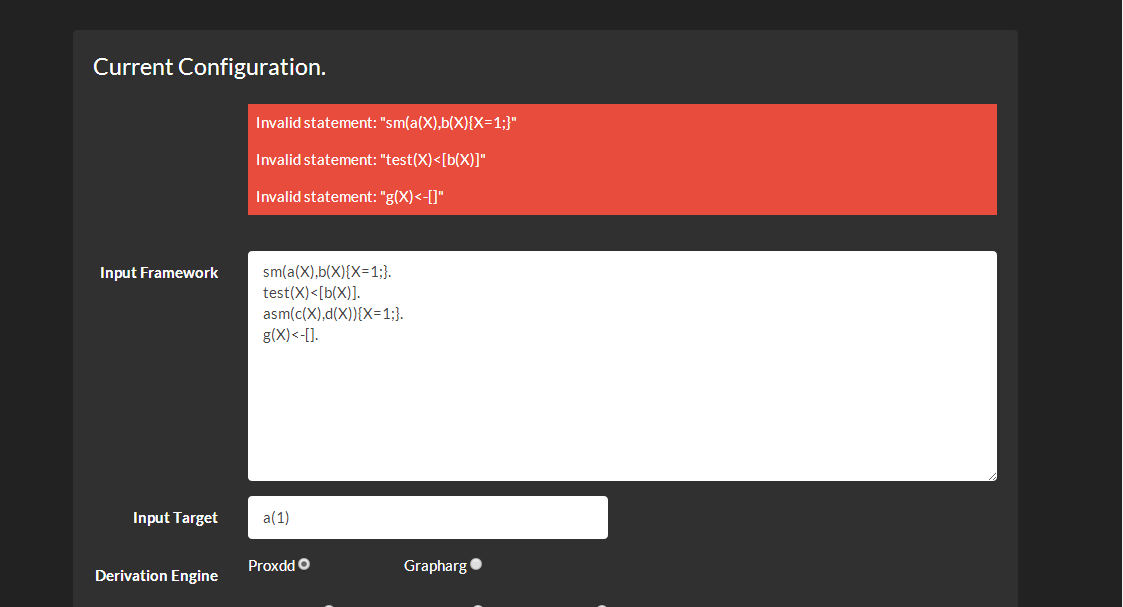
\includegraphics[width=0.8\textwidth]{inputErrors.png}
    \caption{Invalid Statement notifications for the user.}
    \label{fig:invalid_stats}
\end{figure}

\subsection{Validate form of user defined target.}
Additionally, before processing the input the application also verifies that the user defined target is of valid form. This is done by verifying that the target matches a provided regular expressions. The regular expression is defined in [TODO].

\begin{Verbatim}[frame=single]

Target
======
[a-z]?[A-Za-z0-9]+\([a-z0-9][A-Za-z0-9]*
			(,[a-z0-9][A-Za-z0-9]*)*\)

\end{Verbatim}

If the target specified does not match, then it is not of a valid form and the user should correct it. The user is notified of such error by the display of an alert message as shown in [TODO].

\begin{figure}[h]
    \centering
    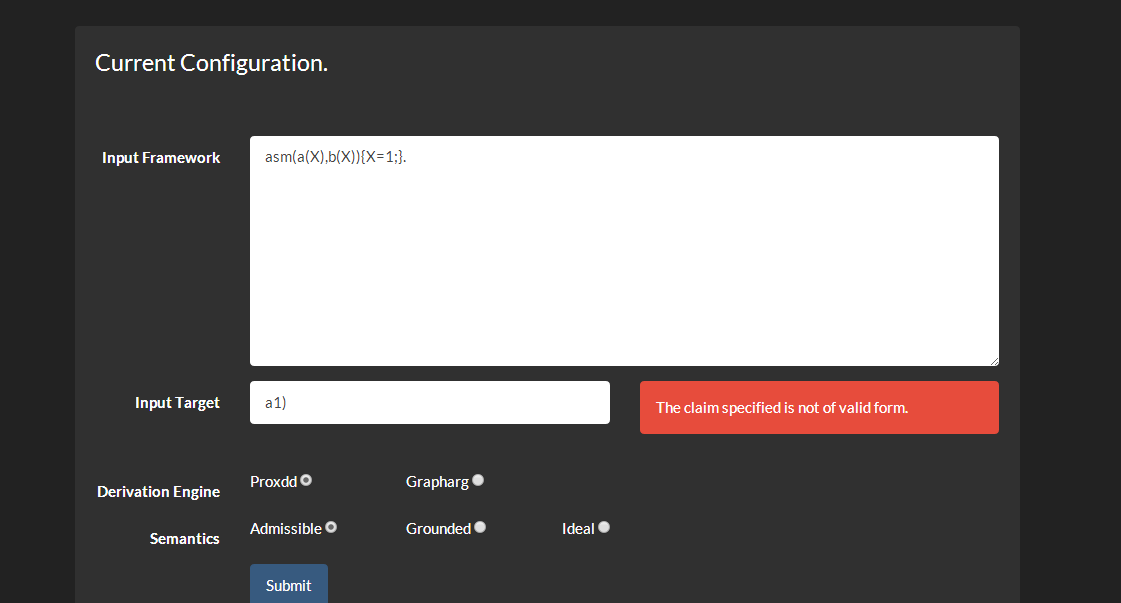
\includegraphics[width=0.8\textwidth]{inputClaimInvalid.png}
    \caption{Input Target is not in a valid format.}
    \label{fig:invalid_claim}
\end{figure}

\subsection{Validate the existence of a target in the grounded framework.}
Taking it a step further our web application's interpreter not only checks if the input of both the target and the framework are syntactically correct, but also provides feedback on whether the target defined is reasonable. Specifically, once the grounded framework has been established the web application then checks whether the target defined by the user exists in the grounded framework.

The implementation searches among the grounded framework for an assumption statement or a rule statement that defines the user provided target. If no such rule exists then the target cannot possibly be reachable withing the current framework. Therefore, a derivation would not be possible.

The user is notified of this case through an alert notification generated and displayed as shown in example [TODO].

\clearpage

\begin{figure}[h]
    \centering
    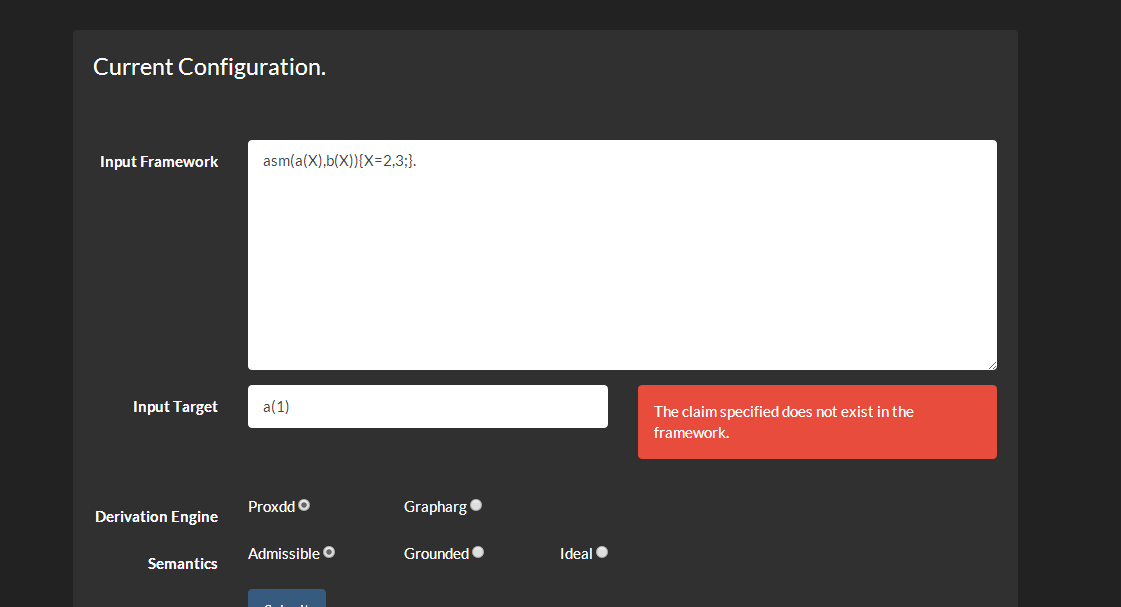
\includegraphics[width=0.8\textwidth]{inputNotFramework.png}
    \caption{Target specified does not exist in framework.}
    \label{fig:not_in_frm}
\end{figure}

\subsection{Check if derivation for target was found.}

Lastly, the system also runs a post-derivation check. This allows us to verify that a derivation has been found for the target once the framework has been processed by the derivation engine. Despite ensuring the validity of the framework and the existence of the target in the grounded framework, it might still be the case that there is no valid derivation for the target under the semantics specified.

This is a perfectly reasonable outcome. Failure to find a solution under specific semantics does not imply that a mistake is made, but rather that no solution is possible to the problem specified. Therefore, it is useful for the user to be informed of this case, as is done in example [TODO].

\clearpage

\begin{figure}[h]
    \centering
    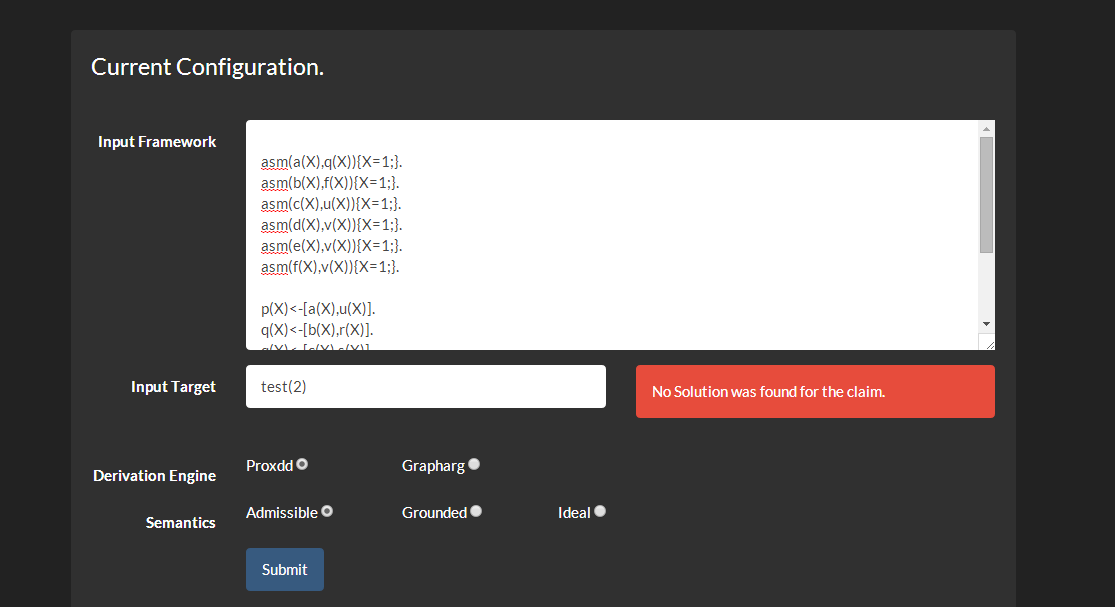
\includegraphics[width=0.8\textwidth]{inputSolNotFound.png}
    \caption{Derivation for target was not found.}
    \label{fig:sol_not_found}
\end{figure}

\section{Example of an input.}

To illustrate a valid input corresponding to a valid ABA framework the following example is provided [TODO].

\begin{framed}
\begin{exmp} Consider a ABA framework as follows:
\\*

\noindent\textbf{R} - includes the following rules:
\\*

\indent	z\textleftarrow a

\indent z\textleftarrow b

\indent y\textleftarrow a

\indent x\textleftarrow d

\indent v\textleftarrow c
\\*

\noindent\textbf{A} = \{a,b,c,d\} and $\bar{a} = z, \bar{b} = y, \bar{c} = x, \bar{d} = v$.

\end{exmp}
\end{framed}

The user can input the framework  above into the web application using the formally defined input language. This can be done be providing the representative list of commands that represent this framework. The input required is provided in section [TODO]. Note that the input provided is in propositional logic and represents an already grounded framework. This is done for readability and the handling of ungrounded frameworks and variables are elaborated on in secton [TODO]. 

[TODO] CHECK THAT THE GROUNDED UNGROUNDED THING IS VALID AT END!

\begin{Verbatim}[frame=single]
asm(a,z).
asm(b,y).
asm(c,x).
asm(d,v).

z <- [a].
z <- [b].
y <- [a].
x <- [d].
v <- [c].
\end{Verbatim}

The input can be provided to the web application through the user interface and the ``Input Framework'' section. This is discussed further in section [TODO], however for illustrative purposes please refer to [TODO] on how this would be achieved.

[TODO] - Image of inputting framework in app.

The user has successfully inserted their framework in the desired format and has additionally declared a valid target. By clicking the ``Submit'' button the input configuration provided is submitted and, provided no error have been found, the web application starts the required procedures to find a valid derivation of the target.

In the case where users desire to specify a domain over which the framework is valid, they can you our language's support of such a case and adapt their commands accordingly. For example consider the framework defined in [TODO], but this time we also want to define the domain over which it is valid (X=1,2). The input to the web application would now be as in [TODO], were we can see the domain being defined in the format \{X=1,2;\} as specified by our formal language.

\begin{Verbatim}[frame=single]
asm(a(X),z(X)){X=1,2;}.
asm(b(X),y(X)){X=1,2;}.
asm(c(X),x(X)){X=1,2;}.
asm(d(X),v(X)){X=1,2;}.

z(X) <- [a(X)].
z(X) <- [b(X)].
y(X) <- [a(X)].
x(X) <- [d(X)].
v(X) <- [c(X)].
\end{Verbatim}